\chapter{Requirements \& Specification}

% [Description of methods used (e.g., use- case diagrams, user stories, use case-descriptions)]

For the CIS 350 project, a use-case diagram along with use-case descriptions were used to define the actors, pre-requisites, and descriptions of the system. 

\section{Use-Cases}

\begin{figure}[htb]
    \centering
    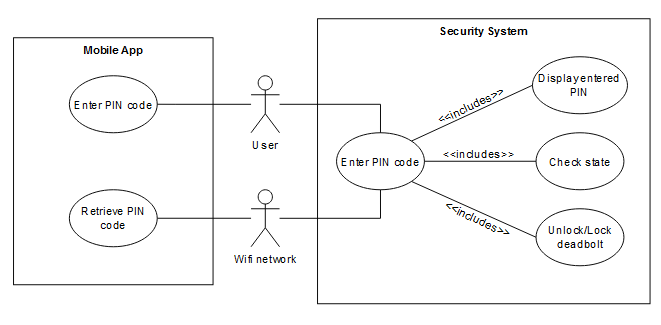
\includegraphics[width = \textwidth]{Images/CIS 350 - Project - Use Case Diagram.png}
    \caption{Project Use-case Diagram}
    \label{fig:Use-case Diagram}
\end{figure}

\newpage \textbf{Use Case Descriptions}

\begin{itemize}
    \item Security System: 
    \begin{itemize}
            \item Actors: User
            \item Pre-requisites: N/A
            \item Use Case Description: The user enters their PIN code on the keypad.
    \end{itemize}

    \item Check State: 
    \begin{itemize}
            \item Actors: User
            \item Pre-requisites: User enters a PIN
            \item Use Case Description: The current state of the lock is referenced to determine if the user has the ability to unlock vs. lock the deadbolt.
    \end{itemize}

    \item Lock/Unlock Deadbolt
    \begin{itemize}
        \item Actors: User
        \item Pre-requisites: Enter PIN and Check State
        \item Use Case Description: The servo is moved in a fashion to either unlock or lock the deadbolt based on the result of the Check State functionality referenced above. 
    \end{itemize}

    \item Display state of lock and entered PIN
    \begin{itemize}
        \item Actors: User
        \item Pre-requisites: Enter PIN
        \item Use Case Description: An LCD will display the status of the lock and if the entered PIN is incorrect. 
    \end{itemize}
    
\end{itemize}

\begin{itemize}
    \item Mobile App (Optional):
        \begin{itemize}
            \item Enter PIN Code
            \begin{itemize}
                \item Actors: User
                \item Pre-requisites: N/A
                \item Use Case Description: The user enters their PIN code on their mobile device. 
            \end{itemize}

            \item Send PIN Code
            \begin{itemize}
                \item Actors: User
                \item Pre-requisites: Enter PIN 
                \item Use Case Description: The Mobile App transmits the entered PIN code to the microcontroller wirelessly and the microcontroller determines if a PIN match has occurred.

            \end{itemize}
        \end{itemize}
\end{itemize}

\newpage \section{Natural Language Requirements}

\begin{itemize}
    \item Req 1. The security system may accept a (Personal Identification Number) PIN code from the user when using the mobile application.
    \item Req 2. The security system may retrieve PIN code from a mobile application when communicating over a Wifi network. 
    \item Req 3. The security system shall accept input from the external keypad when a button is pressed.
    \item Req 4. The security system shall display each number when the user enters them.
    \item Req 5. The security system shall display no more than the four most recently entered PIN digits when input is detected.
    \item Req 6. The security system may display a screensaver when in an idle state.
    \item Req 7. The security system shall determine when the entered code is valid after entry.
    \item Req 8. The security system may determine if a PIN code can be accepted when a key is pressed.
    \item Req 9. The security system shall lock when an invalid code is entered.
    \item Req 10. The security system shall unlock when a valid code is entered.
    \item Req 11. The security system shall display a message when a PIN code is entered.
    \item Req 12. The security system may store multiple unique PIN codes for multiple users.
    
\end{itemize}

\newpage \section{Traceability Matrix}

Table \ref{table: Traceability Matrix} - Traceability Matrix 
\begin{table}[htb]
\begin{tabular}{lccclllllllll}
                                           & \multicolumn{12}{c}{Requirement Number}                                                                                                                                                                                                                                                                      \\ \hline
\multicolumn{1}{|c|}{}                     & \multicolumn{1}{c|}{1} & \multicolumn{1}{c|}{2} & \multicolumn{1}{c|}{3} & \multicolumn{1}{l|}{4} & \multicolumn{1}{l|}{5} & \multicolumn{1}{l|}{6} & \multicolumn{1}{l|}{7} & \multicolumn{1}{l|}{8} & \multicolumn{1}{l|}{9} & \multicolumn{1}{l|}{10} & \multicolumn{1}{l|}{11} & \multicolumn{1}{l|}{12} \\ \hline
\multicolumn{1}{|l|}{Enter Pin (app)}      & \multicolumn{1}{c|}{X} & \multicolumn{1}{c|}{X} & \multicolumn{1}{c|}{}  & \multicolumn{1}{l|}{}  & \multicolumn{1}{l|}{}  & \multicolumn{1}{l|}{}  & \multicolumn{1}{l|}{}  & \multicolumn{1}{l|}{}  & \multicolumn{1}{l|}{}  & \multicolumn{1}{l|}{}   & \multicolumn{1}{l|}{}   & \multicolumn{1}{l|}{X}  \\ \hline
\multicolumn{1}{|l|}{Retrieve Pin Code}    & \multicolumn{1}{c|}{}  & \multicolumn{1}{c|}{X} & \multicolumn{1}{c|}{}  & \multicolumn{1}{l|}{}  & \multicolumn{1}{l|}{}  & \multicolumn{1}{l|}{}  & \multicolumn{1}{l|}{}  & \multicolumn{1}{l|}{}  & \multicolumn{1}{l|}{}  & \multicolumn{1}{l|}{}   & \multicolumn{1}{l|}{}   & \multicolumn{1}{l|}{}   \\ \hline
\multicolumn{1}{|l|}{Enter Pin (hardware)} & \multicolumn{1}{c|}{}  & \multicolumn{1}{c|}{}  & \multicolumn{1}{c|}{X} & \multicolumn{1}{l|}{X} & \multicolumn{1}{l|}{X} & \multicolumn{1}{l|}{}  & \multicolumn{1}{l|}{X} & \multicolumn{1}{l|}{}  & \multicolumn{1}{l|}{}  & \multicolumn{1}{l|}{}   & \multicolumn{1}{l|}{}   & \multicolumn{1}{l|}{X}  \\ \hline
\multicolumn{1}{|l|}{Pin Displayed on LCD} & \multicolumn{1}{l|}{}  & \multicolumn{1}{l|}{}  & \multicolumn{1}{l|}{}  & \multicolumn{1}{l|}{X} & \multicolumn{1}{l|}{X} & \multicolumn{1}{l|}{X} & \multicolumn{1}{l|}{}  & \multicolumn{1}{l|}{}  & \multicolumn{1}{l|}{}  & \multicolumn{1}{l|}{}   & \multicolumn{1}{l|}{X}  & \multicolumn{1}{l|}{}   \\ \hline
\multicolumn{1}{|l|}{Check State}          & \multicolumn{1}{l|}{X} & \multicolumn{1}{l|}{X} & \multicolumn{1}{l|}{}  & \multicolumn{1}{l|}{}  & \multicolumn{1}{l|}{X} & \multicolumn{1}{l|}{}  & \multicolumn{1}{l|}{X} & \multicolumn{1}{l|}{X} & \multicolumn{1}{l|}{X} & \multicolumn{1}{l|}{X}  & \multicolumn{1}{l|}{X}  & \multicolumn{1}{l|}{X}  \\ \hline
\multicolumn{1}{|l|}{Unlock/Lock Deadbolt} & \multicolumn{1}{l|}{}  & \multicolumn{1}{l|}{}  & \multicolumn{1}{l|}{}  & \multicolumn{1}{l|}{}  & \multicolumn{1}{l|}{}  & \multicolumn{1}{l|}{}  & \multicolumn{1}{l|}{}  & \multicolumn{1}{l|}{X} & \multicolumn{1}{l|}{X} & \multicolumn{1}{l|}{X}  & \multicolumn{1}{l|}{}   & \multicolumn{1}{l|}{X}  \\ \hline
\label{table: Traceability Matrix}
\end{tabular}
\end{table}